% Derived geometry at 48 kHz: frame duration N/fs and bin spacing fs/N.
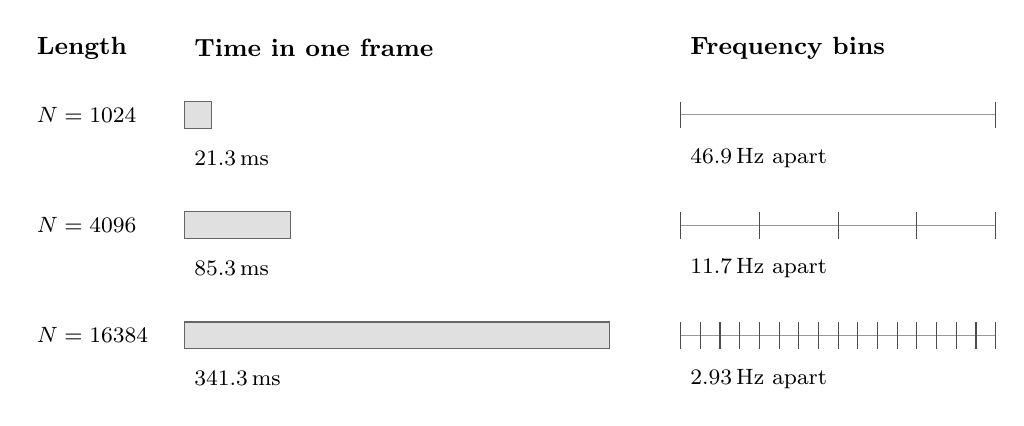
\begin{tikzpicture}[x=1cm,y=1cm,font=\footnotesize]
  \node[anchor=west,font=\small\bfseries] at (0,3.65) {Length};
  \node[anchor=west,font=\small\bfseries] at (2,3.65) {Time in one frame};
  \node[anchor=west,font=\small\bfseries] at (8.3,3.65) {Frequency bins};
  \foreach \n/\intervals/\y in {1024/1/2.8,4096/4/1.4,16384/16/0} {
    \node[anchor=west] at (0,\y) {$N=\n$};
    \pgfmathsetmacro{\duration}{5.4*\intervals/16}
    \draw[fill=black!12,draw=black!60] (2,\y-.17) rectangle +(\duration,.34);
    \draw[black!40] (8.3,\y) -- (12.3,\y);
    \foreach \k in {0,...,\intervals} {
      \pgfmathsetmacro{\x}{8.3+4*\k/\intervals}
      \draw[black!70] (\x,\y-.17) -- (\x,\y+.17);
    }
  }
  \node[anchor=west] at (2,2.25) {$21.3\,\mathrm{ms}$};
  \node[anchor=west] at (2,.85) {$85.3\,\mathrm{ms}$};
  \node[anchor=west] at (2,-.55) {$341.3\,\mathrm{ms}$};
  \node[anchor=west] at (8.3,2.25) {$46.9\,\mathrm{Hz}$ apart};
  \node[anchor=west] at (8.3,.85) {$11.7\,\mathrm{Hz}$ apart};
  \node[anchor=west] at (8.3,-.55) {$2.93\,\mathrm{Hz}$ apart};
\end{tikzpicture}
